\section{Exercise 1 - Mid-depth temperature and \delO{SW} reconstruction}

\subsection{Question 1}
According to \citeauthor{barker2003study} \parencite{barker2003study}, foraminiferal Fe/Mg molar ratios greater than approximately 0.1 are indicative of potential contamination by Mg-rich clay silicates.
Mg/Ca measurements could therefore be rejected if they do not meet the criteria:

\begin{equation} \label{eq:fe_mg}
    \frac{\mathrm{Fe}/\mathrm{Ca}}{\mathrm{Mg}/\mathrm{Ca}} < 0.1 \, \mathrm{mol \cdot mol^{-1}}
\end{equation}

However, visual assessment of the magnitude of potential contamination (Figure \ref{fig:Mg_Fe}) shows that all but one of the eight measurements failing the this criteria are close to the rest of the data in terms of Fe/Mg.
As a result, only the 16.39 ka measurement labelled in Figure \ref{fig:Mg_Fe} is rejected for contamination.

\begin{figure}[h]
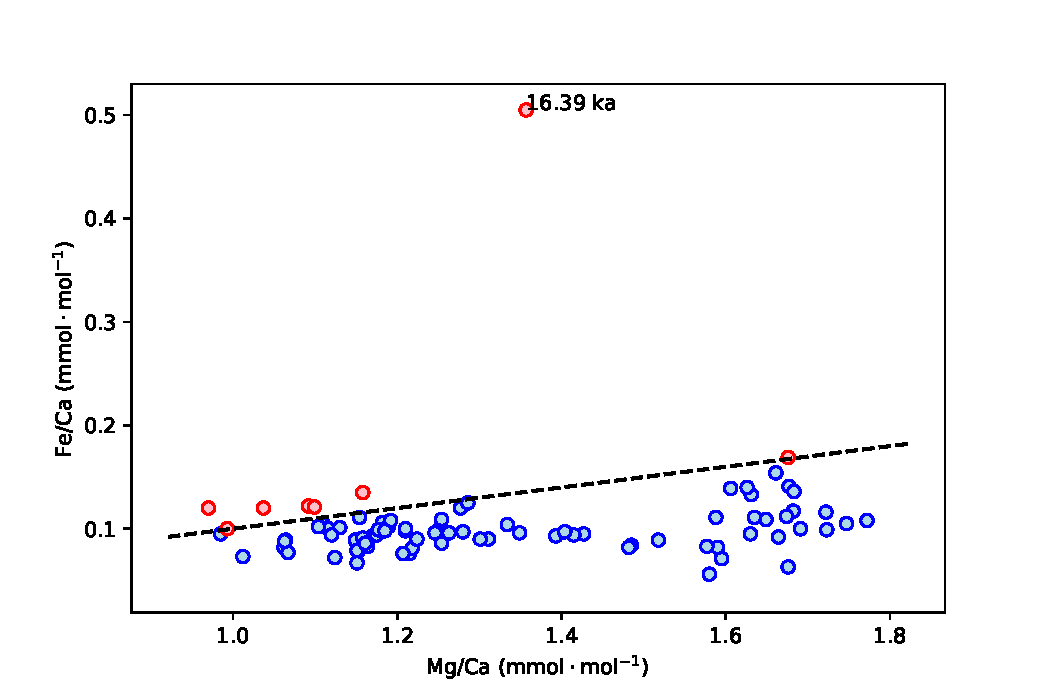
\includegraphics[width=\textwidth]{img/scatter_MgCa_x_FeCa_contaminated.pdf}
    \caption{Ratio of Mg/Ca to Fe/Ca in benthic foraminifera \emph{M. barleeanuum} in RAPiD-10-1P sediment core.
             Dashed line seperates potentially contaminated measurements (red points) according to Equation \ref{eq:fe_mg}.
             Labelled point is identified for rejection.}
        \label{fig:Mg_Fe}
\end{figure}

\subsection{Question 2}

\begin{figure}
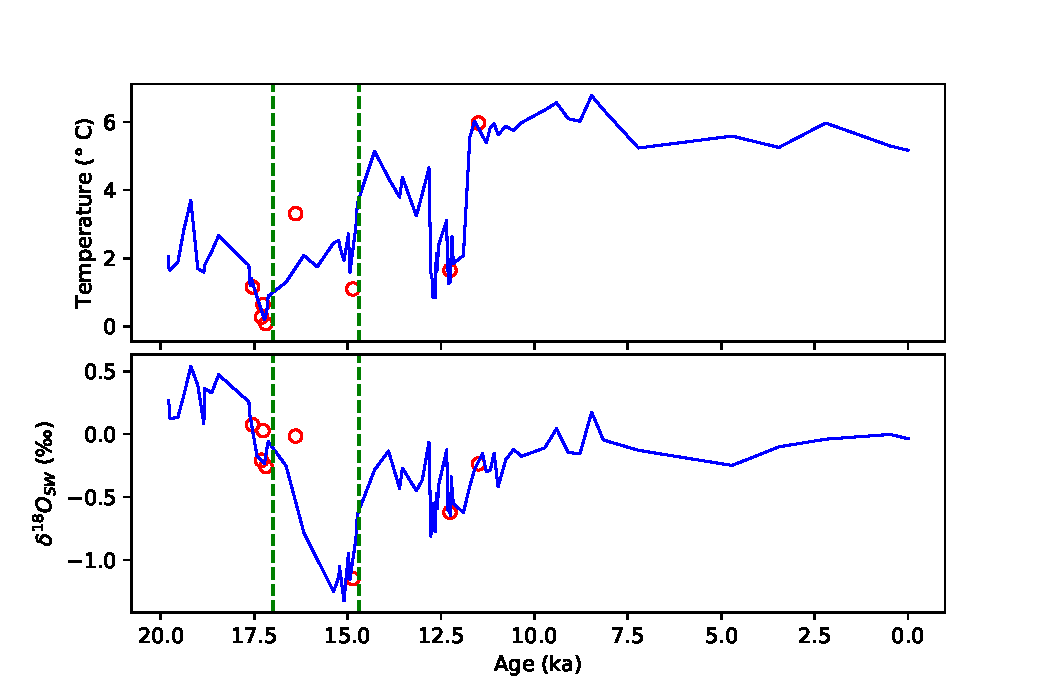
\includegraphics[width=\textwidth]{img/timeseries_temp_and_d18Osw.pdf}
    \caption{The ice-volume corrected oxygen isotope excursion (\delO{SW}) (top) and bottom water temperature determined from Mg/Ca palaeothermetry (bottom) recorded in RAPid-10-1P.
             Red points signify rejected measurements (see text), dashed vertical lines mark approximate boundaries of Heinrich Stadial 1.}
        \label{fig:timeseriestempd18Osw}
\end{figure}
